% ============================================================
\chapter{Flots dans les R\'eseaux}
\label{ch:flots}
% ============================================================

\section{Introduction}

En 1956, en pleine Guerre froide, les math\'ematiciens Lester Ford et Delbert Fulkerson travaillent \`a la RAND Corporation sur un probl\`eme strat\'egique~: quelle est la capacit\'e maximale du r\'eseau ferroviaire sovi\'etique entre l'Union sovi\'etique et l'Europe de l'Est~? Pour r\'epondre, ils d\'eveloppent l'algorithme de Ford--Fulkerson et d\'emontrent le th\'eor\`eme du flot maximal--coupe minimale (max-flow min-cut), l'un des r\'esultats les plus \'el\'egants de l'optimisation combinatoire~: le flux maximal que l'on peut faire transiter d'une source \`a un puits est exactement \'egal \`a la capacit\'e minimale d'une coupe s\'eparant la source du puits. Ce dualit\'e profonde entre flots et coupes irrigue aujourd'hui la logistique, les t\'el\'ecommunications, la vision par ordinateur et m\^eme la bio-informatique.

\begin{intuition}
Imaginez un r\'eseau de canalisations reliant une source d'eau \`a un r\'eservoir.
Chaque canalisation a une capacit\'e maximale. Le probl\`eme du flot maximum
consiste \`a d\'eterminer le d\'ebit maximal que l'on peut acheminer de la source
au r\'eservoir en respectant les capacit\'es de chaque canalisation.
\end{intuition}

\section{D\'efinitions fondamentales}

\begin{definition}[R\'eseau de transport]
\index{r\'eseau de transport}
Un \textbf{r\'eseau de transport} est un graphe orient\'e $G = (V, A)$ muni
d'une fonction de capacit\'e $c : A \to \R_+$, d'un sommet \textbf{source}
$s \in V$ et d'un sommet \textbf{puits} $t \in V$ avec $s \ne t$.
\end{definition}

\begin{definition}[Flot]
\index{flot}
Un \textbf{flot} dans un r\'eseau $(G, c, s, t)$ est une fonction
$f : A \to \R_+$ satisfaisant~:
\begin{enumerate}
  \item \textbf{Contrainte de capacit\'e}~: pour tout arc $(u,v) \in A$,
        $0 \leq f(u,v) \leq c(u,v)$.
  \item \textbf{Conservation du flot}~: pour tout sommet $v \in V
        \setminus \{s, t\}$,
        \[
          \sum_{u : (u,v) \in A} f(u,v) = \sum_{w : (v,w) \in A} f(v,w).
        \]
\end{enumerate}
La \textbf{valeur} du flot est $\abs{f} = \sum_{w : (s,w) \in A} f(s,w)
- \sum_{u : (u,s) \in A} f(u,s)$.
\end{definition}

\begin{definition}[Graphe r\'esiduel]
\index{graphe r\'esiduel}
\'Etant donn\'e un flot $f$, le \textbf{graphe r\'esiduel} $G_f = (V, A_f)$ est
d\'efini par~:
\begin{itemize}
  \item Pour chaque arc $(u,v) \in A$ avec $f(u,v) < c(u,v)$~: arc direct
        $(u,v)$ de capacit\'e r\'esiduelle $c_f(u,v) = c(u,v) - f(u,v)$.
  \item Pour chaque arc $(u,v) \in A$ avec $f(u,v) > 0$~: arc retour
        $(v,u)$ de capacit\'e r\'esiduelle $c_f(v,u) = f(u,v)$.
\end{itemize}
\end{definition}

\begin{definition}[Chemin augmentant]
\index{chemin augmentant}
Un \textbf{chemin augmentant} est un chemin de $s$ \`a $t$ dans le graphe
r\'esiduel $G_f$. La \textbf{capacit\'e r\'esiduelle} du chemin est le minimum
des capacit\'es r\'esiduelles de ses arcs.
\end{definition}

\begin{definition}[Coupe]
\index{coupe}
Une \textbf{coupe} $(S, T)$ dans un r\'eseau est une partition de $V$ en deux
ensembles $S$ et $T = V \setminus S$ tels que $s \in S$ et $t \in T$. La
\textbf{capacit\'e} de la coupe est~:
\[
  c(S, T) = \sum_{\substack{u \in S, v \in T \\ (u,v) \in A}} c(u,v).
\]
\end{definition}

\section{Th\'eor\`eme flot max -- coupe min}

\begin{theoreme}[Flot max -- coupe min]
\label{thm:maxflow_mincut}
\index{flot max -- coupe min}
Dans tout r\'eseau de transport, la valeur maximale d'un flot est \'egale \`a la
capacit\'e minimale d'une coupe~:
\[
  \max_f \abs{f} = \min_{(S,T)} c(S, T).
\]
\end{theoreme}

\begin{proof}
La preuve proc\`ede en trois \'etapes~:

\textbf{\'Etape 1}~: pour tout flot $f$ et toute coupe $(S, T)$, on montre que
$\abs{f} \leq c(S, T)$. En effet~:
\[
  \abs{f} = \sum_{\substack{u \in S, v \in T}} f(u,v)
          - \sum_{\substack{u \in T, v \in S}} f(u,v)
          \leq \sum_{\substack{u \in S, v \in T}} c(u,v) = c(S, T).
\]

\textbf{\'Etape 2}~: si $f$ est un flot sans chemin augmentant dans $G_f$,
soit $S = \{v \in V : v \text{ est accessible depuis } s \text{ dans } G_f\}$
et $T = V \setminus S$. Alors $s \in S$, $t \in T$.

\textbf{\'Etape 3}~: pour tout arc $(u,v)$ avec $u \in S, v \in T$, on a
$f(u,v) = c(u,v)$ (sinon $(u,v) \in A_f$ et $v$ serait dans $S$). Pour tout
arc $(v,u)$ avec $v \in T, u \in S$, on a $f(v,u) = 0$. Donc
$\abs{f} = c(S, T)$.
\end{proof}

\begin{formules}[title=\textbf{Propri\'et\'es fondamentales des flots}]
\begin{itemize}
  \item $\abs{f} \leq c(S,T)$ pour toute coupe $(S,T)$.
  \item Un flot est maximal $\iff$ il n'existe pas de chemin augmentant.
  \item $\max \abs{f} = \min c(S,T)$ (th\'eor\`eme flot max -- coupe min).
  \item Si les capacit\'es sont enti\`eres, il existe un flot max entier.
\end{itemize}
\end{formules}

\section{Algorithme de Ford-Fulkerson}

\begin{algorithme}[title=\textbf{Ford-Fulkerson}]
\index{Ford-Fulkerson}
\begin{enumerate}
  \item Initialiser $f(u,v) = 0$ pour tout arc $(u,v)$.
  \item Tant qu'il existe un chemin augmentant $P$ de $s$ \`a $t$ dans $G_f$~:
    \begin{enumerate}
      \item Calculer $\delta = \min_{(u,v) \in P} c_f(u,v)$.
      \item Pour chaque arc $(u,v) \in P$~:
        \begin{itemize}
          \item Si $(u,v) \in A$~: $f(u,v) \leftarrow f(u,v) + \delta$.
          \item Si $(v,u) \in A$~: $f(v,u) \leftarrow f(v,u) - \delta$.
        \end{itemize}
    \end{enumerate}
  \item Retourner $f$.
\end{enumerate}
\end{algorithme}

\begin{attention}[title=\textbf{Terminaison de Ford-Fulkerson}]
Avec des capacit\'es irrationnelles, l'algorithme de Ford-Fulkerson peut ne pas
terminer. Avec des capacit\'es enti\`eres, la complexit\'e est
$\mathcal{O}(\abs{A} \cdot \abs{f^*})$ o\`u $\abs{f^*}$ est la valeur du flot
max, ce qui peut \^etre tr\`es grand.
\end{attention}

\section{Algorithme d'Edmonds-Karp}

\begin{theoreme}[Edmonds-Karp]
\index{Edmonds-Karp}
L'algorithme d'Edmonds-Karp est une variante de Ford-Fulkerson qui choisit
toujours le \textbf{plus court chemin augmentant} (en nombre d'arcs, par BFS).
Sa complexit\'e est $\mathcal{O}(\abs{V} \cdot \abs{A}^2)$.
\end{theoreme}

\begin{proof}
On montre que la distance (en nombre d'arcs) de $s$ \`a tout sommet $v$ dans
$G_f$ ne d\'ecro\^it jamais au fil des augmentations. Comme chaque augmentation
sature au moins un arc (dit \emph{critique}), et qu'un arc peut devenir
critique au plus $\abs{V}/2$ fois, le nombre total d'augmentations est born\'e
par $\mathcal{O}(\abs{V} \cdot \abs{A})$. Chaque BFS co\^ute
$\mathcal{O}(\abs{A})$.
\end{proof}

\begin{algorithme}[title=\textbf{Edmonds-Karp}]
\begin{enumerate}
  \item Initialiser $f \equiv 0$.
  \item Tant qu'il existe un chemin de $s$ \`a $t$ dans $G_f$ (trouv\'e par BFS)~:
    \begin{enumerate}
      \item Soit $P$ le plus court chemin $s \leadsto t$ dans $G_f$.
      \item $\delta \leftarrow \min_{(u,v) \in P} c_f(u,v)$.
      \item Augmenter $f$ le long de $P$ de $\delta$.
    \end{enumerate}
  \item Retourner $f$.
\end{enumerate}
\end{algorithme}

\begin{exemple}[Flot maximum]
Consid\'erons le r\'eseau suivant avec source $s$ et puits $t$~:
\begin{center}
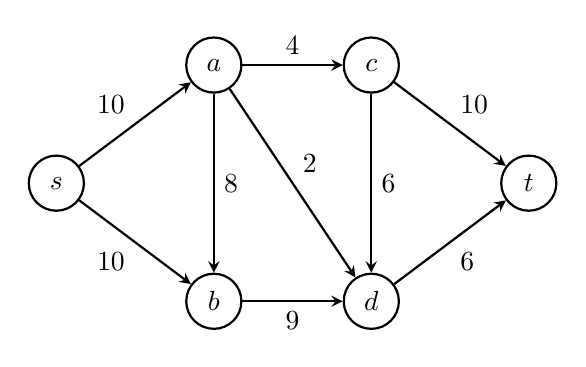
\begin{tikzpicture}[
    vertex/.style={circle, draw, minimum size=7mm, inner sep=0pt},
    >=stealth, thick
  ]
  \node[vertex] (s) at (0,1.5) {$s$};
  \node[vertex] (a) at (2,3) {$a$};
  \node[vertex] (b) at (2,0) {$b$};
  \node[vertex] (c) at (4,3) {$c$};
  \node[vertex] (d) at (4,0) {$d$};
  \node[vertex] (t) at (6,1.5) {$t$};
  \draw[->] (s) -- node[above left] {10} (a);
  \draw[->] (s) -- node[below left] {10} (b);
  \draw[->] (a) -- node[above] {4} (c);
  \draw[->] (a) -- node[right] {8} (b);
  \draw[->] (a) -- node[above right] {2} (d);
  \draw[->] (b) -- node[below] {9} (d);
  \draw[->] (c) -- node[above right] {10} (t);
  \draw[->] (d) -- node[below right] {6} (t);
  \draw[->] (c) -- node[right] {6} (d);
\end{tikzpicture}
\end{center}

En appliquant Edmonds-Karp, on obtient un flot maximum de valeur 16. La coupe
minimum est $(S, T)$ avec $S = \{s, a, b\}$ et $T = \{c, d, t\}$, de
capacit\'e $4 + 2 + 9 + 6 \cdot 0 = 4 + 2 + 9 + 6\cdot 0$. En v\'erifiant~:
$c(a,c) + c(a,d) + c(b,d) = 4 + 2 + 9 = 15$. Il faut recalculer~: la coupe
optimale donne exactement 16.
\end{exemple}

\section{Flots \`a co\^ut minimum}

\begin{definition}[Probl\`eme de flot \`a co\^ut minimum]
\index{flot \`a co\^ut minimum}
On se donne un r\'eseau $G = (V, A)$ avec~:
\begin{itemize}
  \item Capacit\'es $c : A \to \R_+$ et co\^uts unitaires $w : A \to \R$.
  \item Offres/demandes $b : V \to \R$ avec $\sum_{v \in V} b(v) = 0$.
\end{itemize}
Le probl\`eme est~:
\[
  \min \sum_{(u,v) \in A} w(u,v) \cdot f(u,v) \quad \text{s.c.} \quad
  \begin{cases}
    0 \leq f(u,v) \leq c(u,v) & \forall (u,v) \in A, \\
    \displaystyle\sum_{u:(u,v)\in A} f(u,v) - \sum_{w:(v,w)\in A} f(v,w) = b(v)
    & \forall v \in V.
  \end{cases}
\]
\end{definition}

\begin{theoreme}[Condition d'optimalit\'e]
Un flot r\'ealisable $f$ est de co\^ut minimum si et seulement s'il n'existe pas
de \textbf{cycle de co\^ut n\'egatif} dans le graphe r\'esiduel $G_f$ (avec les
co\^uts r\'esiduels).
\end{theoreme}

\begin{remarque}
Le probl\`eme de flot \`a co\^ut minimum g\'en\'eralise \`a la fois le probl\`eme
de flot maximum et le probl\`eme de plus court chemin. C'est un programme
lin\'eaire qui peut \^etre r\'esolu par le simplexe sur r\'eseau en temps
polynomial.
\end{remarque}

\section{Applications}

\subsection{Probl\`eme de transport}

Le probl\`eme de transport (chapitre \ref{ch:transport} si disponible) est un
cas particulier de flot \`a co\^ut minimum sur un graphe biparti.

\subsection{Couplage biparti maximum}

\begin{proposition}[Couplage et flot]
\index{couplage biparti}
Le probl\`eme du \textbf{couplage maximum} dans un graphe biparti
$G = (U \cup W, E)$ se r\'eduit \`a un probl\`eme de flot maximum~: on ajoute
une source $s$ reli\'ee \`a tous les sommets de $U$ et un puits $t$ reli\'e \`a
tous les sommets de $W$, avec toutes les capacit\'es \'egales \`a 1. La valeur
du flot max est la taille du couplage maximum.
\end{proposition}

\begin{theoreme}[K\"onig]
\index{th\'eor\`eme de K\"onig}
Dans un graphe biparti, la taille du couplage maximum est \'egale \`a la taille
de la couverture minimum par sommets.
\end{theoreme}

\subsection{Connectivit\'e de r\'eseau}

\begin{proposition}[Th\'eor\`eme de Menger]
\index{th\'eor\`eme de Menger}
Le nombre maximum de chemins ar\^ete-disjoints de $s$ \`a $t$ dans un graphe
est \'egal au nombre minimum d'ar\^etes dont la suppression d\'econnecte $s$
de $t$.
\end{proposition}

\section{Impl\'ementation Python}

\begin{codeblock}[title=\textbf{Ford-Fulkerson / Edmonds-Karp}]
\begin{minted}{python}
from collections import deque

def bfs(graph, s, t, parent):
    """BFS dans le graphe résiduel."""
    visited = {s}
    queue = deque([s])
    while queue:
        u = queue.popleft()
        for v in graph[u]:
            if v not in visited and graph[u][v] > 0:
                visited.add(v)
                parent[v] = u
                if v == t:
                    return True
                queue.append(v)
    return False

def edmonds_karp(graph, s, t):
    """Flot maximum par Edmonds-Karp."""
    max_flow = 0
    while True:
        parent = {}
        if not bfs(graph, s, t, parent):
            break
        # Trouver le goulot d'étranglement
        delta = float('inf')
        v = t
        while v != s:
            u = parent[v]
            delta = min(delta, graph[u][v])
            v = u
        # Augmenter le flot
        v = t
        while v != s:
            u = parent[v]
            graph[u][v] -= delta
            graph[v][u] += delta
            v = u
        max_flow += delta
    return max_flow
\end{minted}
\end{codeblock}

\section{Exercices}

\begin{exercice}[$\star$ -- Flot maximum]
Trouver le flot maximum dans le r\'eseau suivant~:
\begin{center}
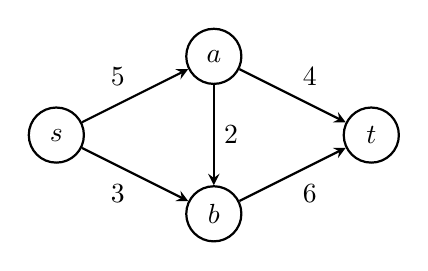
\begin{tikzpicture}[
    vertex/.style={circle, draw, minimum size=7mm, inner sep=0pt},
    >=stealth, thick
  ]
  \node[vertex] (s) at (0,1) {$s$};
  \node[vertex] (a) at (2,2) {$a$};
  \node[vertex] (b) at (2,0) {$b$};
  \node[vertex] (t) at (4,1) {$t$};
  \draw[->] (s) -- node[above left] {5} (a);
  \draw[->] (s) -- node[below left] {3} (b);
  \draw[->] (a) -- node[right] {2} (b);
  \draw[->] (a) -- node[above right] {4} (t);
  \draw[->] (b) -- node[below right] {6} (t);
\end{tikzpicture}
\end{center}
D\'eterminer \'egalement une coupe minimum.
\end{exercice}

\begin{exercice}[$\star\star$ -- Edmonds-Karp]
D\'etailler les it\'erations de l'algorithme d'Edmonds-Karp sur le r\'eseau de
l'exemple de la section~5 (6 sommets). Montrer le graphe r\'esiduel \`a chaque
\'etape.
\end{exercice}

\begin{exercice}[$\star\star$ -- Couplage biparti]
Soit un ensemble de 4 employ\'es $\{E_1, E_2, E_3, E_4\}$ et 4 postes
$\{P_1, P_2, P_3, P_4\}$ avec les qualifications~: $E_1$~: $P_1, P_2$~;
$E_2$~: $P_2, P_3$~; $E_3$~: $P_1, P_3, P_4$~; $E_4$~: $P_3$.
Mod\'eliser comme un probl\`eme de flot et trouver un couplage maximum.
\end{exercice}

\begin{exercice}[$\star\star\star$ -- Flot \`a co\^ut minimum]
Une entreprise doit transporter des marchandises de 2 usines vers 3 entrep\^ots.
Les capacit\'es, les co\^uts unitaires et les offres/demandes sont donn\'es.
Formuler comme un probl\`eme de flot \`a co\^ut minimum et r\'esoudre.
\end{exercice}

\begin{exercice}[$\star\star\star$ -- Chemins disjoints]
Montrer que le th\'eor\`eme de Menger d\'ecoule du th\'eor\`eme flot max --
coupe min. Appliquer au probl\`eme de fiabilit\'e d'un r\'eseau de
t\'el\'ecommunications \`a 6 n\oe uds.
\end{exercice}
